\documentclass[twoside,twocolumn,11pt]{article} %If no option is specified, 10pt is assumed
\DeclareUnicodeCharacter{202F}{FIX ME!!!!} % latex is a problem child
\usepackage{blindtext} % Package to generate dummy text throughout this template 
\usepackage[sc]{mathpazo} % Use the Palatino font
\usepackage[T1]{fontenc} % Use 8-bit encoding that has 256 glyphs
\linespread{1.05} % Line spacing - Palatino needs more space between lines
\usepackage{microtype} % Slightly tweak font spacing for aesthetics
\usepackage{csquotes}
\usepackage[english]{babel} % Language hyphenation and typographical rules
\usepackage{graphicx}
\usepackage{float}
\usepackage[linguistics]{forest}
\usepackage{wrapfig}
\usepackage{amsmath,amssymb}
\usepackage{graphicx}
\usepackage{subcaption}

\usepackage[hmarginratio=1:1,top=32mm,columnsep=20pt,margin=0.6in]{geometry} % Document margins, margin=0.6in wasn't there first.
\usepackage[labelfont=bf,textfont=it]{caption} % Custom captions under/above floats in tables or figures
\usepackage{lettrine} % The lettrine is the first enlarged letter at the beginning of the text
\usepackage{enumitem} % Customized lists
\setlist[itemize]{noitemsep} % Make itemize lists more compact
\usepackage{abstract} % Allows abstract customization
\renewcommand{\abstractnamefont}{\normalfont\bfseries} % Set the "Abstract" text to bold
\renewcommand{\abstracttextfont}{\normalfont\small\itshape} % Set the abstract itself to small italic text
\usepackage{titlesec} % Allows customization of titles
\renewcommand\thesection{\Roman{section}} % Roman numerals for the sections
\renewcommand\thesubsection{\roman{subsection}} % roman numerals for subsections
\titleformat{\section}[block]{\large\scshape\centering}{\thesection.}{1em}{} % Change the look of the section titles
\titleformat{\subsection}[block]{\large}{\thesubsection.}{1em}{} % Change the look of the section titles
\usepackage{fancyhdr} % Headers and footers
\pagestyle{fancy} % All pages have headers and footers
\fancyhead{} % Blank out the default header
\fancyfoot{} % Blank out the default footer
\fancyhead[C]{Electrical Steel: An investigation into the
brittleness of the Fe-Si alloy} % Custom header text
\fancyfoot[RO,LE]{\thepage} % Custom footer text
\usepackage{titling} % Customizing the title section
\usepackage{cite}
\usepackage{hyperref} % For hyperlinks in the PDF
\setlength{\headheight}{13.59999pt} % make fancyheader stop complaining
%----------------------------------------------------------------------------------------
%	TITLE SECTION
%----------------------------------------------------------------------------------------
\setlength{\droptitle}{-4\baselineskip} % Move the title up
\pretitle{\begin{center}\Huge\bfseries} % Article title formatting
\posttitle{\end{center}} % Article title closing
\title{Radiopropa: Hybrid minimizer} % Article title
\author{%
\textsc{Arthur Adriaens} \\[1ex] % Your name
\normalsize Ghent University \\ % Your institution
\normalsize \href{mailto:arthur.adriaens@ugent.be}{arthur.adriaens@ugent.be} % Your email address
}

\date{\today} % Leave empty to omit a date
\renewcommand{\maketitlehookd}{%
\begin{abstract}
\noindent 
This is an alternative module to the iterative raytracer to make use of the
radiopropa module.  It succeeds in more rapidly tracing the path from the event
to the detector and also arrives closer to the detector as the final result is
not limited by the final drawn sphere size but by a given tolerence.
\end{abstract}
}

%----------------------------------------------------------------------------------------

\begin{document}

% Print the title
\maketitle

%----------------------------------------------------------------------------------------
%	ARTICLE CONTENTS
%----------------------------------------------------------------------------------------
\section{Introduction}
The Hybrid ray tracer, in the source code called the "hybrid minimizer" is the
result of the first semester of my masters thesis. Upon learning that more
complex ice models where needed and after seeing the work that has been done to
iteratively ray trace a path \cite{2022icrc.confE1027O}, I checked out the source
code to try and understand the workings. In the source code I saw that a clever but 
unsuccesful attempt was made to implement the scipy.optimize module as an alternative
to the iterative ray tracer. I came up with a way to implement this 
that succeeded as will be explained below.
\section{How it works}
\begin{figure*}
	\centering
	\includegraphics[width=\textwidth]{figures/explanation.png}
	\caption{explanation of the hybrid method}
	\label{fig:explanation}
\end{figure*}
The hybrid minimizer can be seen as an extension of the iterative raytracer, it
checks after the first loop (as explained in the paper by B. Oeyen et al.
\cite{2022icrc.confE1027O}) if there are 2 distinct launch regions, if this is
the case it breaks out of the loop 
as is visually explained using a modified version of B. Oeyen et al. their figure in
figure \ref{fig:explanation}. 
It then goes on to use the scipy.optimize.minimize module
to find the solutions in the respective angle intervals
as shown in figure \ref{fig:explscipy} (minimizing $\Delta z$). If it doesn't find 2
distinct regions after the first loop, it falls back on the iterative ray tracer. 
\begin{figure}
	\centering
	\includegraphics[width=0.6\textwidth]{figures/PrincipleHybridIllu.pdf}
	\caption{explanation of scipy.optimize.minimize}
	\label{fig:explscipy}
\end{figure}
\section{random number generator}
To test the hybrid minimizer the numpy random module was used to generate
random , the considered square (as there is only a z component to the
ice model the 3D problem is essentially only a 2D problem) is x:0.1km,4km and
z:-0.1km,-3km.\footnote{This was to get around issues concerning events that 
won't even trigger in a full simulation}
\section{Performance Optimalisation}
\subsection{Length of the normal vector}
As visually explained in figure \ref{fig:normexpl}, the size of the normal vector
influences how big the ray tracer's step size is taken close to the detector. This
thus influences the convergence and time taken. The results of varying this are shown
in figures \ref{fig:norminfl} and \ref{fig:norminfl2}.
The first optimization conclusion is thus: take the normal vector length to be 1 meter.
\subsection{ztol}
We'll now change the tolerence on the vertical distance away from the detector which is deemed
accepted i.e in figure \ref{fig:normexpl} if $\Delta z$ is below this threshold it's accepted.
The results are shown in figures \ref{fig:ztolinfl} and \ref{fig:ztolinfl2}.
From which we can conclude the second optimization conclusion: take ztol to be 0.05 m.
\subsection{Sphere Size \& Step Size}
As explained in Oeyen et al.'s work, the initial rays are sent out in steps of a
certain angle and with a sphere around the detector (as can also be seen in
figure \ref{fig:explanation}, but for clarification I again refer to their
paper). The sphere size and step size weren't jet optimized. But as
this is the slowest step in the hybrid ray tracer this was optimized here (only
the initial sphere and step size as those are relevant for the hybrid
raytracer) as seen in figure .

\begin{figure*}
\begin{minipage}{0.49\textwidth}
	\centering
	\includegraphics[width=1.1\textwidth]{figures/hybrid_comparison_N_1000.pdf}
	\caption{Hybrid}
	\label{fig:acchyb}
\end{minipage}
\begin{minipage}{0.49\textwidth}
	\centering
	\includegraphics[width=1.1\textwidth]{figures/iterative_comparison_N_1000.pdf}
	\caption{Iterative}
	\label{fig:accit}
\end{minipage}
\end{figure*}

\begin{figure}
	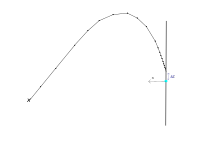
\includegraphics[width=0.5\textwidth]{figures/PrincipleNormIllu.pdf}
	\caption{how normal vector size influences the stepsize}
	\label{fig:normexpl}
\end{figure}
\begin{figure}
	\centering
	\begin{minipage}{\textwidth}
		\includegraphics[width=0.5\textwidth]{figures/NormVsTime.pdf}
	\end{minipage}
	\begin{minipage}{\textwidth}
		\includegraphics[width=0.5\textwidth]{figures/NormVsSigmaTime.pdf}
	\end{minipage}
\caption{influence of the lenth of the normal vector}
\label{fig:norminfl}
\end{figure}
\begin{figure}
	\begin{minipage}{\textwidth}
		\includegraphics[width=0.5\textwidth]{figures/NormVsTime.pdf}
	\end{minipage}
	\begin{minipage}{\textwidth}
		\includegraphics[width=0.5\textwidth]{figures/NormVsSigmaAZ.pdf}
	\end{minipage}
\caption{influence of the lenth of the normal vector}
\label{fig:norminfl2}
\end{figure}

\begin{figure}
	\begin{minipage}{\textwidth}
		\includegraphics[width=0.5\textwidth]{figures/ZtolVsTime2.pdf}
	\end{minipage}
	\begin{minipage}{\textwidth}
		\includegraphics[width=0.5\textwidth]{figures/ZtolVsSigmaTime.pdf}
	\end{minipage}
\caption{influence of the tolerence on vertical distance}
\label{fig:ztolinfl}
\end{figure}
\begin{figure}
	\begin{minipage}{\textwidth}
		\includegraphics[width=0.5\textwidth]{figures/ZtolVsTime2.pdf}
	\end{minipage}
	\begin{minipage}{\textwidth}
		\includegraphics[width=0.5\textwidth]{figures/ZtolVsSigmaAZ.pdf}
	\end{minipage}
\caption{influence of the tolerence on vertical distance}
\label{fig:ztolinfl2}
\end{figure}

\begin{figure}
	\includegraphics[width=0.5\textwidth]{figures/SphereAndStepAll.pdf}
	\caption{Variation in Sphere and Step size with report on relative time.}
	\label{fig:SphereStepInfl}
\end{figure}

%----------------------------------------------------------------------------------------
%	REFERENCE LIST
%----------------------------------------------------------------------------------------
\bibliography{sources}
\bibliographystyle{plain}

%----------------------------------------------------------------------------------------

\end{document}
